\section{InfluxDB}\label{section:influxdb}
\paragraph{Time Series} In mathematics, a time series is a series of data points which are indexed (or listed or graphed) in time order (see~\ref{fig:random time-series}).
More generally, a time series is a sequence taken at evenly spaced intervals over a period of time. As a result, it's a sequence of discrete-time data.
% \todo{EB: verificare ``succession''} DG: come alternative propongo sequence
Ocean tidal heights, sunspot counts, and the Dow Jones Industrial Average's daily closing value are all examples of time series.
\begin{figure}[ht]
    \centering
    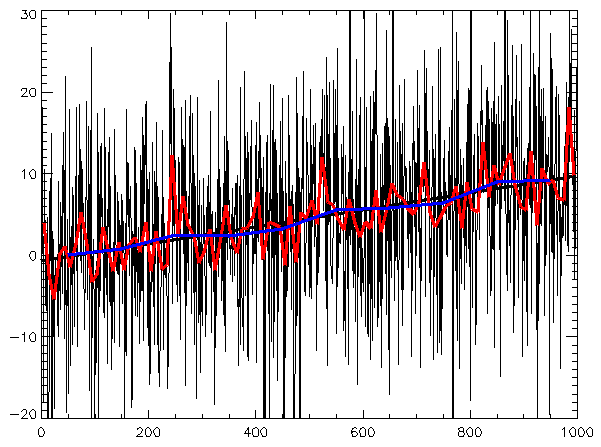
\includegraphics[width=.9\textwidth]{content/chapter_3/images/random-data-plus-trend-r2.png}
    \caption{Random data plus trend, with best-fit line and different smoothing applied. (Source: Wikimedia Commons~\cite{file:random-data-plus-trend-r2})}
    \label{fig:random time-series}
\end{figure}
\subsection{TSDB: time series database}
It follows that a time series database \acs{tsdb} is a software system that is designed to store and serve this peculiar type of data, time series, using time(s) and value(s) pairs(s).
Timescale, popular \ac{tsdb}, CEO \textit{Ajay Kulkarni}~\cite{Misc:asay_why_time_series} put it:
\begin{quote}
    Time-series datasets track changes to the overall system
    as INSERTs, not UPDATEs.
    This practice of recording each and every change to the system as a new, different row is what makes time-series data so powerful.
    It allows us to measure change: analyse how something changed in the past, monitor how something is changing in the present, predict how it may change in the future.

    So, here's how I like to define time-series data: data that collectively represents how a system/process/behaviour changes over time.
\end{quote}
Although it is possible to store time-series data in many diverse database types, the design of these systems with \textbf{time} as a \textbf{key} index is distinctly different from relational databases, which reduces discrete relationships through referential models.
In many cases, the repositories of time-series data will utilize compression algorithms to manage the data efficiently~\cite{Book:devops_cookbook}. Furthermore, time series databases can also be configured to regularly delete old data, unlike traditional databases which are designed to store data indefinitely.

\subsection{Influx solution}
InfluxDB is an open-source time series database \acs{tsdb} created by the InfluxData organization~\cite{Misc:influxdata_website}.
It is written in the Go programming language and is used for time series data storage and retrieval in various sectors such as operations monitoring, application metrics, \acl{IoT}, and, especially important in our context, sensor data and real-time analytics.
It also supports the processing of data from Graphite, a data logging and graphing tool for time series data~\cite{Misc:thegraphiteproject_2021_graphite}.
% \todo{EB: ci vorrebbe forse una reference a Graphite}

\paragraph{Core Features}
InfluxDB has no external dependencies and provides a SQL-like vocabulary with built-in time-centric functions for querying a data structure made up of measurements, series, and points, which listens on port 8086~\cite{Misc:influx_docs}.

\begin{table}[ht]
    \centering
    \begin{tabular}{|l|l|l|l|l|}
        \toprule
        Time                 & location & scientist  & butterflies & honeybees \\ \midrule
        2015-08-18T00:00:00Z & 1        & langstroth & 12          & 23        \\ \hline
        2015-08-18T00:00:00Z & 1        & perpetua   & 1           & 30        \\ \hline
        2015-08-18T00:06:00Z & 1        & langstroth & 11          & 28        \\ \hline
        2015-08-18T05:54:00Z & 2        & langstroth & 2           & 11        \\ \hline
        2015-08-18T06:00:00Z & 2        & langstroth & 1           & 10        \\ \hline
        2015-08-18T06:06:00Z & 2        & perpetua   & 8           & 23        \\ \hline
        2015-08-18T06:12:00Z & 2        & perpetua   & 7           & 22        \\ \bottomrule
    \end{tabular}
    \caption{Sample time series dataset: number of butterflies and honeybees counted by two scientists}\label{tab:influx_example}
\end{table}

Each point is made up of a fieldset and a timestamp, which are key-value pairs. These pairs form a series when they are grouped together by a set of key-value pairs known as a tagset. Finally, a measurement is created by grouping series together using a string identification.
64-bit integers, 64-bit floating points, strings, and booleans are among the possible values as shown in Table~\ref{tab:influx_example}. The time and tag set are used to sort the points.
As a side note it is important to know that data is downsampled and removed according to retention policies, which are set by measurement and that \textit{Continuous Queries} are executed on a regular basis and the results are stored in a goal measurement.

\paragraph{Design Tradesoff}
InfluxDB is a time series database and, by this aspect, has several limitations; as a matter of fact,
% In fact Indeed 
being optimized for this use case involves a number of trade-offs, primarily to increase performance at the cost of functionality~\cite{Misc:influx_docs}.
Below, it is reported a list of three design ideas that lead to compromises that I personally encountered during my experience:
% \todo{DG: Potrebbero essere più di 3, mi sembrava un buon compromesso}
\begin{enumerate}
    \item Deletes are a rare occurrence. When they do occur, it is almost always against large ranges of old data that are cold for writes.
    \item Updates to existing data are a rare occurrence, and contentious updates never happen. Time series data is predominantly new data that is never updated.
    \item Many time series are ephemeral. There are often time series that appear only for a few hours and then go away, e.g., a new host that gets started and reports for a while and then gets shut down.
\end{enumerate}
\begin{table}[ht]
    \begin{tabularx}{\textwidth}{>{\raggedright\arraybackslash\parskip1ex}X@{\kern4\tabcolsep}>{\raggedright\arraybackslash\parskip1ex}X}
        \toprule
        \hfil\bfseries Pros
         &
        \hfil\bfseries Cons
        \\\cmidrule(r{3\tabcolsep}){1-1}\cmidrule(l{-\tabcolsep}){2-2}
        %% PROS, separated by empty line or \par
        Restricting access to deletes and updates allows for increased query and write performance\par
        InfluxDB is good at managing discontinuous data\par
         &
        %% CONS, separated by empty line or \par
        Delete and Update functionality is significantly restricted, since InfluxDB is not \acs{crud} \par
        Schema-less design means that some database functions are not supported e.g. there are no cross table joins\par
        \\\bottomrule
    \end{tabularx}
    \caption{Pros and cons of InfluxDB}
\end{table}
\paragraph{Conclusion}
It is therefore not surprising to conclude that, when compared to a general purpose relational database like SQL Server, InfluxDB, using default single node configuration, 
outperformed both write speed, disk storage usage (by a factor of 27x) and query execution time, where InfluxDB is up to 20x faster with an average of 8x faster~\cite{Misc:noor_2017_universit}.
It can be seen that InfluxDB, tailored-made for Time Series data, is released after other competitive technologies (like Graphite, TimescaleDB, Prometeus) and yet still 1st among the popularity tier list\footnote{\url{https://db-engines.com/en/ranking_trend/time+series+dbms}}.
% \todo{EB: riscrivere contentuto che possa essere fruibile anche se stampato}
The InfluxQL, SQL-subset query language, helps make it easier to use and adapt for people who are used to working with relational databases such as MySQL, even though influx
implementation is a smaller subgroup, not fully supporting \ac{crud} operations. For more complex queries is almost mandatory using Flux, a functional-like query language developed in-house by Influx~\cite{Misc:influx_docs}.
